\newpage
\section{User Interface}
\label{sec:chapter_2_section_4}

Per definizione software CAD, è un acronimo inglese usato per indicare due concetti correlati, ma differenti:
\begin{itemize}
  \item Computer-Aided Drafting;
  \item Computer-Aided Design;
\end{itemize}
L'applicazione web che si è implementata si presente come un software CAD semplificato, dove la
user interface comprende una user interface:
\begin{itemize}
  \item 2D canvas (come si evince dalla Figura~\ref{fig:view2D})
  \item 3D canvas (come si evince dalla Figura~\ref{fig:viewer3D}).
\end{itemize}
Dalla toolbar lo user pu\`o accedere alle funzionalit\`a relative a: ciclo di vita del progetto (new, save, load);
view/interaction mode switching (2D, 3D); interaction mode changing (selecting, pan, zoom).
Il canvas \`e un area nella quale lo user pu\`o interagire con il data modello attuale. Nella modalit\`a 2D
il modello \`e visualizzato come una proiezione 2D dall'alto, e l'interazione consiste nell'inserimento, selezione e modifica
dell'elemento (in accordo con le specifiche interattive del prototipo). Nella modalit\'a 3D un modello 3D pu\`o essere
inspezionato e navigato, rispettivamente attraverso il trackball o l'interazione in prima persona, mentre gli oggetti
possono essere scelti consentendo la selezione dell'elemento.
La sidebar visualizza le propriet\`a dell'elemento correntemente selezionato. Nel pannello delle propriet\`a \`e possibile
vedere la descrizione dell'elemento, aggiungere/rimuovere metadata, e modificare qualsiasi propriet\`a.
Quest'ultima modalit\'a di interazione consente allo user di associare annotazioni semantiche su ogni parte del modello.
\newpage

\subsection{Viewer 2D}
Il \emph{2D-viewer} invoca il \emph{2Dgf} degli elementi costruiti e aggiunti al modello e genera un suo output usando
gli elementi SVG.
Per far fronte ai frequenti aggiornamenti provenienti dall'interazione con il disegno da parte dell'utente,
sfrutta la \emph{Virtual DOM}~\cite{vdom}, che permette di aggiornare solo la parte modificata evitando così
il completo rendering della scena. Per eseguire le operazioni di pan e zoom, tipicamente necessaria in questo
tipo di strumento, sviluppiamo un componente ad-hoc
di React denominato \emph{ReactSVGPanZoom}\footnote{\url{https://github.com/chrvadala/react-svg-pan-zoom}}.\\

% The \emph{2D-viewer} invokes the \emph{2Dgf} of the building elements added to the model and renders its output using SVG
% elements. To cope with frequent updates coming from the user drawing interaction, it exploits the \emph{Virtual DOM}~\cite{vdom},
%  which permits to update only the modified part thus avoiding complete redrawing of the scene. To perform pan and zoom operations,
%   typically necessary in this kind of tool, we develop an ad-hoc React component named
  % \emph{ReactSVGPanZoom}\footnote{https://github.com/chrvadala/react-svg-pan-zoom}.

\begin{figure}[htbp] %  figure placement: here, top, bottom, or page
   \centering
   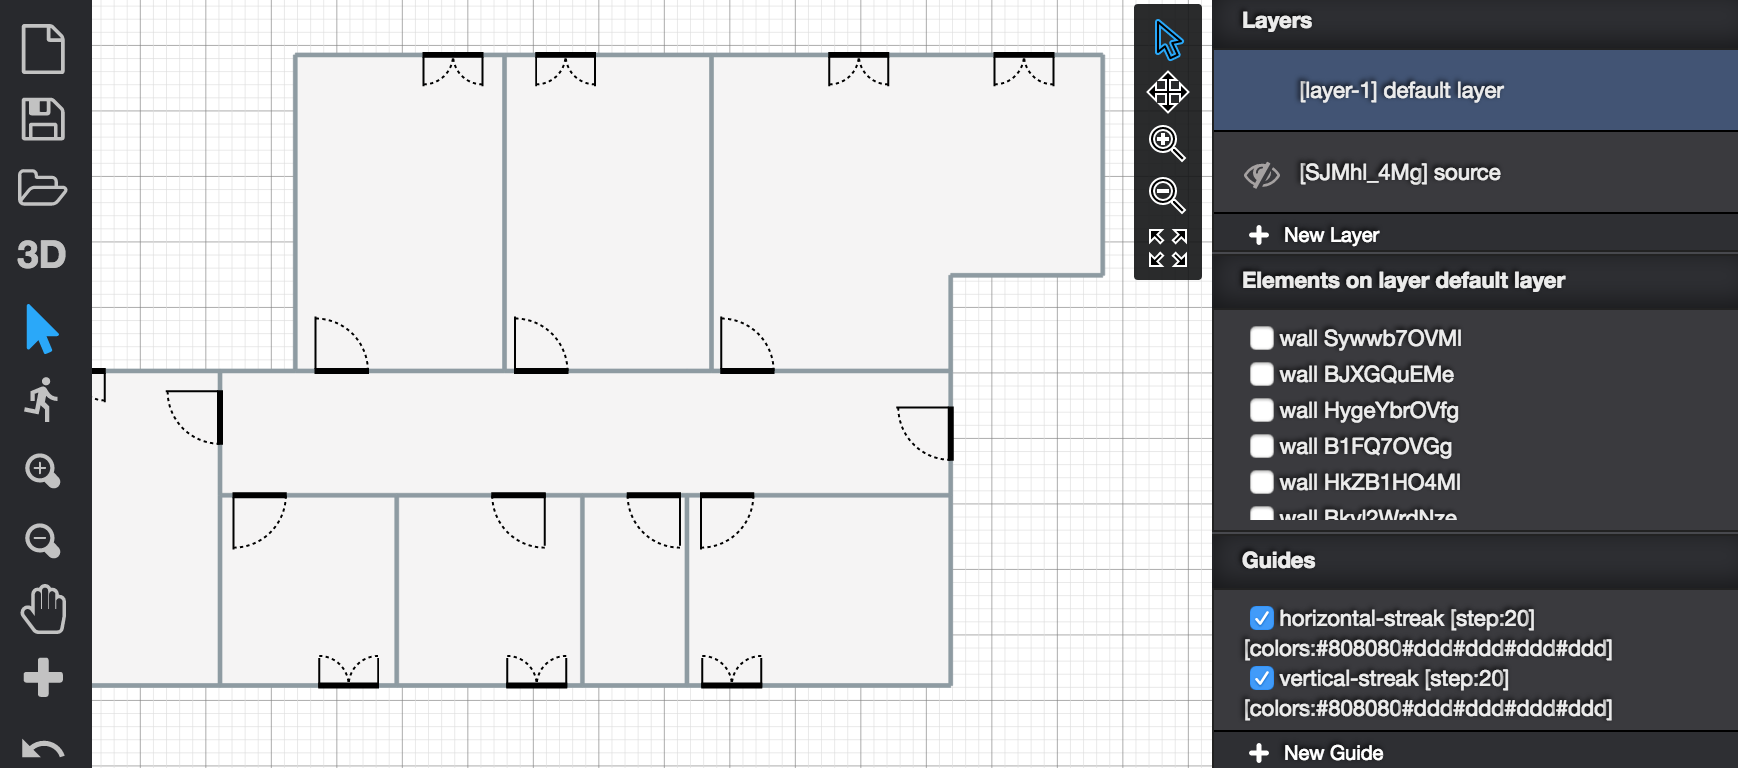
\includegraphics[width=1\linewidth]{images/2d}
   \caption{Schermata viewer 2D}
   \label{fig:view2D}
\end{figure}
\newpage


\subsection{Viewer 3D}
Il \emph{3D-viewer} invoca il \emph{3Dgf} dagli elementi di costruzione aggiungi al model e lo renderizza in output usando
le primitive WebGL\emph{Three.js}~\footnote{\url{https://threejs.org/}}. \`E stato implementato un \emph{diff} e \emph{patch} di
sistema, standardizzate in ~\cite{rfc6902}: gli oggetti Three.js sono associati con elementi costruttivi all'interno
dello Stato, in modo che ogni volta che l'utente attiva un'azione che si traduce in una modifica dello stato,
l'applicazione calcola la differenza tra il vecchio stato e quello nuovo e cambia solo l'oggetto interessato.
In particolare possiamo avere le seguenti \textit{operazioni}:
\begin{itemize}
  \item \emph{add};
  \item \emph{replace};
  \item \emph{remove};
\end{itemize}

% The \emph{3D-viewer} invokes the \emph{3Dgf} of the building elements added to the model and renders its output using WebGL
%  primitives via \emph{Three.js}~\footnote{https://threejs.org/}. It has been implemented a \emph{diff} and \emph{patch}
%  system, standardized in~\cite{rfc6902}: Three.js objects are associated with building elements inside the state, so every
%   time the user triggers an action that results in a state alteration, the application computes the difference between the
%    old state and the new one and changes only the affected object. In particular we can have the following \textit{operations}:
%     (i) \emph{add}, (ii) \emph{replace} and (iii) \emph{remove}.

\begin{figure}[htbp] %  figure placement: here, top, bottom, or page
   \centering
   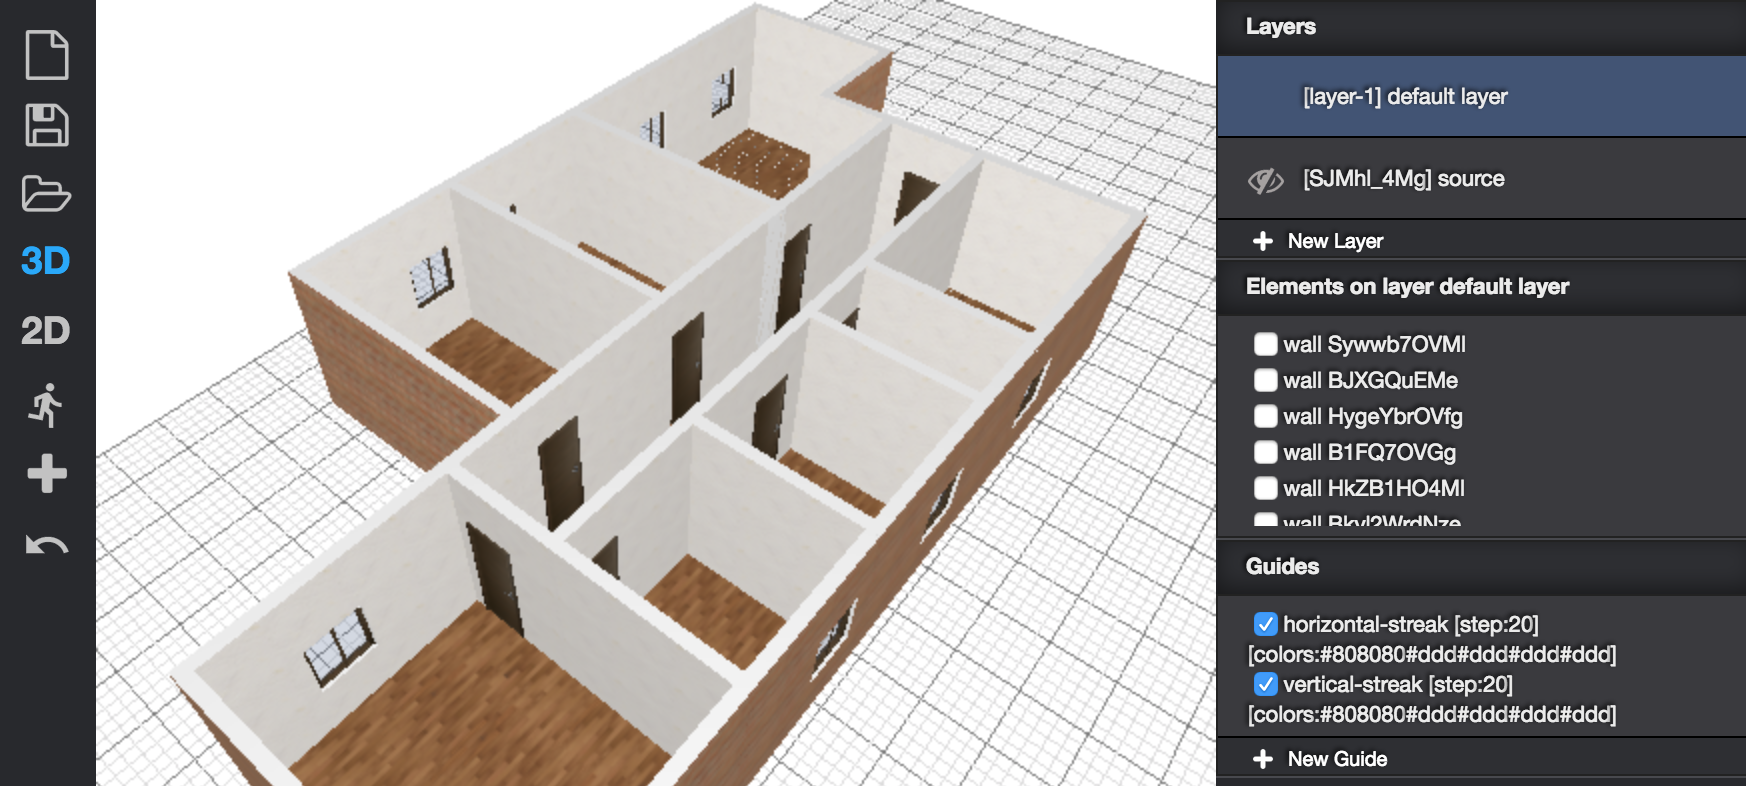
\includegraphics[width=1\linewidth]{images/3d}
   \caption{Schermata viewer 3D }
   \label{fig:viewer3D}
\end{figure}
\newpage
